\section{相对同调}
\sourcepage{56--57}
设 $K_0$ 为复形 $K$ 的子复形。在拓扑学的许多应用中，考虑所谓 $K$ 模 $K_0$ 的相对同调群很方便。这里先简要介绍并计算一些例子，把更完整的讨论留到第三章。

链群 $C_p(K_0)$ 可以自然地视为 $C_p(K)$ 的子群。形式上说，若 $c_p$ 是 $K_0$ 上的链，即定义在 $K_0$ 的定向单形上的函数，可令其在 $K$ 中所有不属于 $K_0$ 的定向 $p$ 维单形上取值 $0$，从而扩张为 $K$ 上的链。若把 $c_p$ 写成 $K_0$ 的定向单形的线性组合，则只需将这些单形也视为属于 $K$，就把 $c_p$ 视为了 $K$ 的链。

\entry{定义}{1.10.1}若 $K_0$ 为 $K$ 的子复形，称 $(K,K_0)$ 为\textbf{单纯偶}（simplicial pair），上下文清楚时也简称为\textbf{偶}。商群
\[
C_p(K)/C_p(K_0)
\]
称为 $K$ 模 $K_0$ 的\textbf{相对链群}，记为 $C_p(K,K_0)$。

注意，$C_p(K,K_0)$ 是自由阿贝尔群。事实上，给 $K$ 的各 $p$ 维单形定向，得到 $C_p(K)$ 的一组基；其中由 $K_0$ 的定向 $p$ 维单形组成的子族是 $C_p(K_0)$ 的基。因此商群自由，其一组基由所有形如
\[
\{\sigma_i\}=\sigma_i+C_p(K_0)
\]
的陪集组成，其中 $\sigma_i$ 是 $K$ 中不属于 $K_0$ 的 $p$ 维单形。

边界算子 $\partial:C_p(K_0)\to C_{p-1}(K_0)$ 就是 $C_p(K)$ 上边界算子的限制。在不致混淆时，用同一符号表示它们。这个同态诱导相对链群间的同态 $C_p(K,K_0)\to C_{p-1}(K,K_0)$，也记作 $\partial$。与前面一样，$\partial\circ\partial=0$。令
\[
\begin{aligned}
Z_p(K,K_0)&=\ker\bigl(\partial:C_p(K,K_0)\to C_{p-1}(K,K_0)\bigr),\\
B_p(K,K_0)&=\operatorname{im}\bigl(\partial:C_{p+1}(K,K_0)\to C_p(K,K_0)\bigr),\\
H_p(K,K_0)&=Z_p(K,K_0)/B_p(K,K_0).
\end{aligned}
\]
这三个群分别称为 $K$ 模 $K_0$ 的\textbf{相对 $p$ 维闭链群}、\textbf{相对 $p$ 维边界链群}与\textbf{第 $p$ 相对同调群}。

相对 $p$ 维链是陪集 $c_p+C_p(K_0)$；它是相对闭链，当且仅当 $\partial c_p$ 由 $K_0$ 承载。它是相对边界，当且仅当存在 $K$ 的某条 $(p+1)$ 维链 $d_{p+1}$，使 $c_p-\partial d_{p+1}$ 由 $K_0$ 承载。

\entry{例}{1.10.2}设 $K$ 由某个 $n$ 维单形及其各面组成，$K_0$ 由其真面组成。则除 $p=n$ 时 $C_p(K,K_0)$ 为无限循环群外，其他维数的相对链群都为零。因此
\[
H_i(K,K_0)=0\quad(i\ne n),\qquad H_n(K,K_0)\cong\Z.
\]
\entry{例}{1.10.3}设 $K$ 为复形，$K_0$ 只由 $K$ 的一个顶点 $v$ 组成。利用第 1.8 节的结果，容易看出 $H_0(K,v)$ 自由阿贝尔：从 $|K|$ 中除包含 $v$ 的分支之外的每个分支中，选取一个顶点，就得到一组基。因此 $H_0(K,v)\cong\widetilde H_0(K)$。

对于 $p>0$，也不难证明 $H_p(K,v)\cong H_p(K)$，见习题。\translatornote{原文此处左边带有约化符号 $\widetilde H_p(K,v)$，但相对约化群尚未定义；在正维中使用普通相对同调即可。}

\sourcepage{58}
\entry{例}{1.10.4}设 $K$ 为图 1.10.1 的复形，其底空间为正方形区域，$K_0$ 为底空间等于正方形边界的子复形。容易看出，$2$ 维链 $\sum m_i\sigma_i$ 代表相对闭链，当且仅当 $m_1=m_2=m_3=m_4$。因为二维没有非零边界，所以 $H_2(K,K_0)\cong\Z$，链 $\gamma=\sum\sigma_i$ 代表一个生成元。
\begin{center}
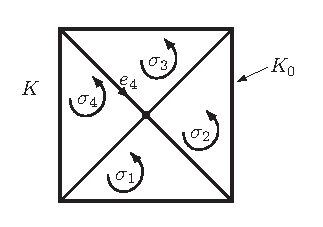
\includegraphics[width=58mm]{figures/1-10-1.pdf}\\图 1.10.1
\end{center}
例 1.6.13 已证明，$K$ 中任意 $1$ 维链 $c$ 都同调于由 $K_0\cup e_4$ 承载的链 $c_3$。若 $c$ 代表相对 $1$ 维闭链，即 $\partial c$ 由 $K_0$ 承载，则 $\partial c_3=\partial c$ 也由 $K_0$ 承载。所以 $c_3$ 在 $e_4$ 上的值必须为零，即 $c_3$ 实际上由 $K_0$ 承载。因此 $H_1(K,K_0)=0$。将此计算与例 1.10.2 比较，使尚待证明的“相对同调群是拓扑不变量”这一断言更为可信。

\entry{例}{1.10.5}设 $K$ 为图 1.10.2 的复形，其底空间称为\textbf{环带}（annulus）。令 $K_0$ 为底空间等于 $K$ 的内外两条边界之并的一维复形。计算 $K$ 模 $K_0$ 的同调。
\begin{center}
\begin{minipage}{.47\textwidth}\centering
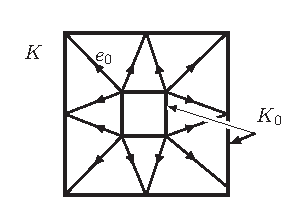
\includegraphics[width=56mm]{figures/1-10-2.pdf}\\图 1.10.2
\end{minipage}\hfill
\begin{minipage}{.47\textwidth}\centering
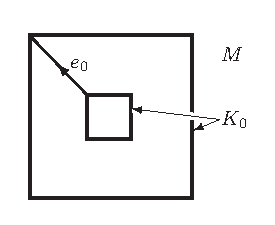
\includegraphics[width=51mm]{figures/1-10-3.pdf}\\图 1.10.3
\end{minipage}
\end{center}
首先，$H_0(K,K_0)=0$，因为零维相对链群本身就为零。计算 $H_1,H_2$ 之前，先验证三个事实：
\begin{enumerate}[label=(\roman*)]
\item 若 $c$ 为 $K$ 的 $1$ 维链，则它同调于由图 1.10.3 中子复形 $M$ 承载的某条 $1$ 维链。
\item 给 $K$ 的所有 $2$ 维单形逆时针定向。若 $d$ 为 $K$ 的任意 $2$ 维链，且 $\partial d$ 由 $M$ 承载，则 $d=m\gamma$，其中 $\gamma$ 为所有定向 $2$ 维单形的和。
\item $\partial\gamma$ 由 $K_0$ 承载。
\end{enumerate}
令 $e_0$ 为图 1.10.2 中的定向 $1$ 维单形。因为 $\partial e_0$ 位于 $K_0$，所以 $e_0$ 代表相对 $1$ 维闭链。由 (i)，任意相对 $1$ 维闭链都相对同调于 $\{e_0\}$ 的某个整数倍。而这样的非零相对闭链不会是相对边界。事实上，若对于 $K$ 的某条 $2$ 维链 $d$，$ne_0-\partial d$ 由 $K_0$ 承载，则 $\partial d$ 由 $M$ 承载，由 (ii) 得 $d=m\gamma$。再由 (iii)，$\partial d=m\partial\gamma$ 由 $K_0$ 承载，所以 $n=0$。因此
\[
H_1(K,K_0)\cong\Z,
\]
相对闭链 $e_0$ 代表一个生成元。利用 (ii)、(iii) 作类似论证，可得 $H_2(K,K_0)\cong\Z$，相对闭链 $\gamma$ 代表一个生成元。

\sourcepage{59--60}
学生常把 $H_p(K,K_0)$ 理解为：将 $|K_0|$ 压缩为一点 $p$ 而得商空间 $X=|K|/|K_0|$ 后，所得空间模该点的同调。若 $X$ 同胚于多面体，因而其单纯同调有定义，这种理解确实正确，但证明并不容易，见引理 8.10.1 及第 4.13 节习题。

粗略地说，$H_p(K,K_0)$ 只依赖于 $K$ 中位于 $K_0$ 之外或其边界上的部分，而忽略 $K_0$ 内部的部分。下面正式表述这个事实。

\entry{定理}{1.10.6（切除定理）}设 $K$ 为复形，$K_0$ 为子复形。设 $U$ 是包含在 $|K_0|$ 中的开集，且 $|K|\setminus U$ 是 $K$ 的某个子复形 $L$ 的多胞体。令 $L_0$ 为多胞体等于 $|K_0|\setminus U$ 的子复形。则包含映射诱导同构
\[
H_p(L,L_0)\cong H_p(K,K_0).
\]
可将 $(|L|,|L_0|)$ 视为从 $|K|,|K_0|$ 中切除开集 $U$ 而得，见图 1.10.4。
\begin{center}
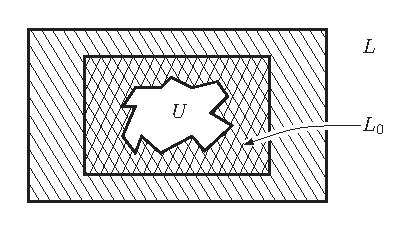
\includegraphics[width=73mm]{figures/1-10-4.pdf}\\图 1.10.4
\end{center}
\noindent\textbf{证明：}考虑复合映射
\[
\varphi:C_p(L)\longrightarrow C_p(K)\longrightarrow C_p(K)/C_p(K_0),
\]
即先包含再投影。$\varphi$ 为满射，因为商群的一组基由所有不属于 $K_0$ 的 $\sigma_i$ 的陪集 $\{\sigma_i\}$ 组成，而 $L$ 包含所有这些单形。$\varphi$ 的核恰为 $C_p(L_0)$。所以对所有 $p$，它诱导同构
\[
C_p(L)/C_p(L_0)\cong C_p(K)/C_p(K_0).
\]
边界算子在此同构下保持不变，故 $H_p(L,L_0)\cong H_p(K,K_0)$。\hfill$\square$

这个初等事实有一些有用的推论，后面将讨论。

\subsection*{习题}
\begin{enumerate}
\item 设 $K$ 为图 1.10.2 的复形，$K_1$ 为其外边界。计算 $H_i(K)$ 与 $H_i(K,K_1)$。
\item 设 $K$ 的底空间为 Möbius 带，$K_0$ 为其边界。计算 $H_i(K)$ 与 $H_i(K,K_1)$。\translatornote{本题原文后一个群写作 $H_i(K,K_1)$，但只定义了 $K_0$；应为 $H_i(K,K_0)$。}［提示：见例 1.4.6，此时边界由线段 $ab,bc,cd,de,ef,fa$ 组成。］
\item 证明：若 $K$ 为复形，$v$ 为其顶点，则对所有 $i$ 有 $H_i(K,v)\cong\widetilde H_i(K)$。［提示：$i=1$ 时需要小心。］
\item 描述一般情况下的 $H_0(K,K_0)$。
\item 用通常的带标记矩形表示环面 $|K|$，令 $K_0$ 为矩形上边所表示的子复形。计算 $H_i(K,K_0)$。［见图 1.7.4，$|K_0|$ 是线段 $ab,bc,ca$ 的并。］
\item 设 $K$ 为二维复形，$\sigma$ 为其一个 $2$ 维单形，$K_0$ 为底空间等于 $|K|\setminus\Int\sigma$ 的子复形。计算 $H_i(K,K_0)$。
\end{enumerate}
